\section{Passwörter}
\begin{frame}{Passwörter}
  \visible<+->{Wer hat mindestens fünf Online-Accounts?}

  \visible<+->{Wer hat dafür mindestens drei verschiedene Passwörter?}

  \visible<+->{Wer beachtet, Passwörter nur über HTTPS einzugeben?}
\end{frame}

\begin{frame}{Anzahl Passwörter}
  \begin{itemize}
    \item Zugangsdaten von Diensteanbietern werden bei Hackerangriffen gestohlen
    \begin{itemize}
      \item Angreifer versuchen, die Zugangsdaten auch bei anderen Anbietern zu verwenden
      \item Schaden lässt sich begrenzen, wenn Benutzername und Passwort nur bei diesem einen Anbieter passen
    \end{itemize}
    \item Besonders wichtig: E-Mail-Accounts
    \begin{itemize}
      \item Weil ,,Passwort zurücksetzen`` oft via E-Mail
      \item Wer den E-Mail Account übernommen hat,\\ kann dadurch sämtliche Accounts übernehmen
    \end{itemize}
    \item Ideal: Jedes Passwort nur einmal verwenden
    \item Alternative: Passwörter ,,salzen``
    \begin{itemize}
      \item \textit{passwort}.amz für Onlineshop a
      \item \textit{passwort}.zal für Onlineshop z
      \item \textit{anderespasswort} für Mails
    \end{itemize}
  \end{itemize}
\end{frame}

\begin{frame}{Passwort Wiederverwertung}
  \begin{center}
    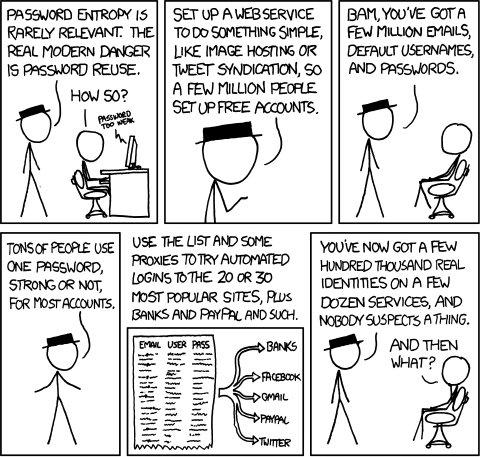
\includegraphics[height=0.8\textheight]{images/password_reuse_top.png}\\
  \end{center}
  \tiny Bildquelle: Ausschnitt aus \href{http://xkcd.com/792/}{xkcd: Password Reuse / CC BY-NC 2.5}
\end{frame}

\begin{frame}{Sichere Passwörter}
  \begin{block}{Anforderungen}
  \begin{itemize}
    \item Klein- und Großbuchstaben, Zahlen,\\ begrenzt: Sonderzeichen
    \item Wichtiger: Lang genug!
  \end{itemize}
  \end{block}
  \begin{block}{Merkbarkeit}
  \begin{itemize}
    \item Pass\textit{satz} statt Passwort\\
      Beispiel: \texttt{margaretthatcheris110\%SEXY}\\
      \scriptsize (aus Snowden-Interview: \url{https://www.youtube.com/watch?v=yzGzB-yYKcc})
      \normalsize
    \item würfeln, dann sieben zufällige Wörter verwenden\\
      \scriptsize siehe \url{https://theintercept.com/2015/03/26/passphrases-can-memorize-attackers-cant-guess/}
  \end{itemize}
  \end{block}
\end{frame}

\begin{frame}{Passwort-Manager}
  \begin{block}{Passwort-Manager}
    Passwort-Manager verwalten Passwörter in einer verschlüsselten Datenbank; der Anwender muss sich idealerweise nur das Datenbank-Passwort merken.
  \end{block}
  \begin{columns}
    \begin{column}{.5\textwidth}
      \pause
      \textbf{Vorteile}
      \begin{itemize}
        \small
        \item erzeugt statistisch zufällige Passwörter
        \item ermöglicht es,\\jedes Passwort\\nur einmal zu verwenden
      \end{itemize}
    \end{column}
    \begin{column}{.5\textwidth}
      \pause
      \textbf{Nachteil}
      \begin{itemize}
        \small
        \item Eingefangene Malware\\bekommt alle Passwörter\\auf einmal
      \end{itemize}
    \end{column}
  \end{columns}
  ~\\
  \pause
  \textbf{Anmerkungen}
  \begin{itemize}
    \small
    \item Entscheidung zwischen lokalen und ``Cloud''-Datenbanken\\ = ``klassischer'' Tradeoff zwischen Sicherheit und Komfort
    \item Backups machen -- und wichtige Passwörter trotzdem merken!
    \item unsere Empfehlung: KeePass(X)
  \end{itemize}
\end{frame}

\endinput
